\documentclass[10pt,twocolumn,letterpaper]{article}

\usepackage{amsmath}
\usepackage{alltt}
\usepackage{amssymb}
\usepackage{chemfig}
\usepackage{mathtools}
\usepackage{listings}
\usepackage{wrapfig}
\usepackage{color}
\usepackage{float}
\usepackage{caption}
\usepackage{subcaption}
\usepackage{paralist}
\usepackage{tcolorbox}
\usepackage{braket}
\usepackage[framemethod=TikZ]{mdframed}
\usepackage[english]{babel}
\usepackage[utf8x]{inputenc}
\usepackage{esint}
\usepackage{hyperref}
\hypersetup{
    colorlinks=true,
    linkcolor=blue,
    filecolor=magenta,      
    urlcolor=cyan,
}

\title{DASS End Semester}
\date{2020-04-26}
\author{Kalp Shah : 2018113003}

\setlength{\columnsep}{20pt}

\begin{document}
\pagenumbering{arabic}
\maketitle
\begin{abstract}
The Indian Government has imposed a country wide lockdown, due to the 
pandemic created by Corona Virus (COVID 19). This move was required, 
and to end this pandemic the guidlines given must be followed. But many 
people are not following it, and these people need to be caught. Our 
sofware system is the one that utilizes the current infrastructure and 
uses face recognition to detect people and penalize them as required.

\end{abstract}

\section*{Introduction}
Corona Virus (COVID 19) has created a global pandemic as it is a virus with 
mortality rate of over 4\%, having already killed millions of people worldwide 
and spreads via air and contact and to add to the problem at hand, there is no 
cure in sight. Hence, the global lockdown needs to be obeyed for the pandemic 
to be over.

\section*{Literature Review}
There are many studies going on to find the cure of the Corona Virus, each 
looking at the similarity in structure of the virus with that of SARS COV (also 
known as Corona Virus), and trying to make a cure by modifying drugs made 
for the original Corona Virus.
\\\\
Detailed study on the structure of the virus is also carried out, which 
enables people to know what preventive measures to apply. For example, the 
lipid bilayer which is essential for the survival of the virus can be killed 
using soap. This information was known after knowing the structure and formation 
of the virus.
\\\\
Software companies like Google and Apple are probiding technologies that can, 
using bluetooth, that can do contact tracing (Corona spreads via contact) and 
is also providing APIs that can do the same.
\\\\
These are some of the ways in which many leading scientists and sofware 
companies are helping fighting the Corona Virus.

\section*{System Architecture}
The software solution proposed in the paper is completely software based with 
no extra hardware infrastructure required and can be implemented without 
any modifications.

\subsection*{Concept}
The concept behind the idea is that people behave more when a monetary penalty is 
associated with the negative result. Hence, if a person is barred from going outside 
with the penalty of say Rs. 5000, they will not do it unless absolutely necassary.
Of course if there is a genuine reason of going outside, no penalty will be applicable.
\\\\
The idea is to monitor the amount of time spent by each person out of their 
homes and penalise (monetary) accordingly with the option for them to appeal the 
penalty within reason.

\subsection*{Pipeline}
The pipeline of the system is as follows:\\\\ There are many cameras on every crossroads 
in India, and are already used to find culprits who are not wearing helmets (or 
other such trafic violations) and memos are sent to their house. The same structure 
can be used to monitor vehicles and people.\\\\ Everytime the camera detects a person, 
it gets updated on the database managed for each person uniquely identified 
using the Adhaar card  information (Which has both, the photo of the person and the 
identification of the vehicles owned under the persons name).\\\\After that every 
weekend, a memo is sent which contains the amount of money default. People can 
also see the total amount they owe using a webpage which uses Adhaar ID as the 
login information and also gives an option to appeal the penalty online. \\\\
The person can then pay via the portal provided in the web application. The 
person can pay the amount wanted, which will be deducted from the total amount 
owed.\\\\After that, every person who is eligible (Government employed) to 
review complaints will be alloted the complaints which they have the 
power to waive off.\\\\
This is the basic working of the application.

\subsection*{Users}
The users of the application are :
\begin{itemize}
    \item The Defalters \\
        People who check their amount, complain and pay.
    \item Employee (Type 1) \\
        The people who review the complaints.
    \item Employee (Type 2)\\
        The people who send out the memos.
\end{itemize}
As the whole system is automated no third party is required.

\subsection*{MVC}

\subsubsection*{Model}
The model in this system is the database that stores the amount of times the person 
is detected by the camera, the amount they owe and the complaints 
from the user.

\subsubsection*{View}
The view is the web application that displays the amount
(of times detected) and default amount after the user logs in using their 
Adhaar ID.

\subsubsection*{Controller}
The controller is the application that monitors the cameras 
to detect which person is detected, the user who can complain and the 
employee who can review the complaint.

\subsubsection*{Interactions}
There are two ways by which a controller would update the model, which would in turn 
lead to the view being updated. The ways are :

\begin{itemize}
    \item Contoller detects a person, then it identifies the person using either their 
    photograph or using their vehicle ID, and using that ID, updates the amount seen by 
    1, which then results in the amount owed feild also being changed.
    \item Controller wants to complain against an offence against it, which leads to the 
    model updating the complaint feild.
    \item Controller pays amount which is deducted from the amount due and is updated in 
    the model. 
    \item Controller reviews the complaint, and if deems resonable can waive off the 
    amount which will update the database and deduct the amount.
\end{itemize}

Every change in model leads to change in view.

\subsection*{Updation of the Database}
Database is updated when the controller intercts with the model. The instances 
of the same are given above. No other method can change the database.

\subsection*{Diagrams}
\subsubsection*{Class Diagram}
\begin{figure}[h]
    \centering
    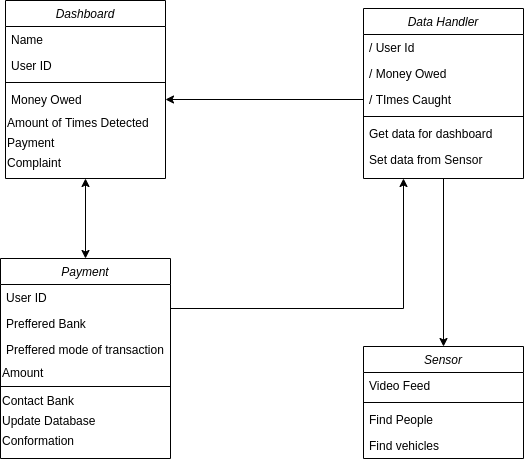
\includegraphics[scale=0.3]{img/Class Diagram.png}    
    \caption{Class Diagram}
\end{figure}

\noindent This diagram gives a basic idea on how the classes are generated 
and how they will correspond with each other.
\\\\
The classes created are :
\begin{itemize}
    \item Dashboard\\
    The frontend of the web application that displays information, is a gateway to 
    payment, and house the method to give complaints.
    \item Data Hander\\
    Handles the database and allows different classes to access and modify it.
    \item Payment\\
    Payment portal that takes necessary information from the user takes him to the 
    banks website for payment and reports if the transaction was successful.
    \item Sensor\\
    Automated machine that detects and updates database when it encounters and 
    identifies a person.
    \item Review Panel\\
    A panel that assigns complaints to each user who is an employee and gives 
    it the option to accept and reject the complaint.
    \item Complaint Panel \\
    Query panel that allows people to add complaints opposing the penalty.
\end{itemize}

\subsubsection*{Sequence Diagram}
\begin{figure}[h]
    \centering
    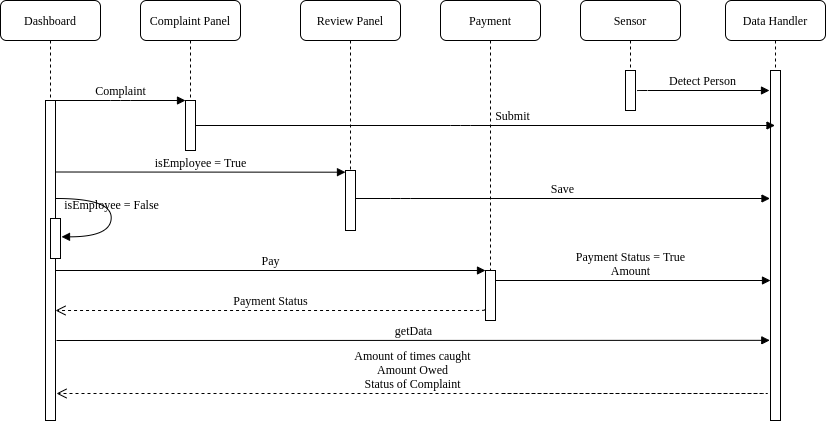
\includegraphics[scale=0.3]{img/Sequence Diagram.png}    
    \caption{Sequence Diagram}
\end{figure}

\noindent Diagram given in Figure 2 describes all the possible sequences that can exist while 
operating the software system.

\subsubsection*{State Diagrams}
Below are the state diagrams of the more important processes of the 
software system. These conatin complaint, payment, review and sensing itself.\\
\begin{figure}[h]
    \centering
    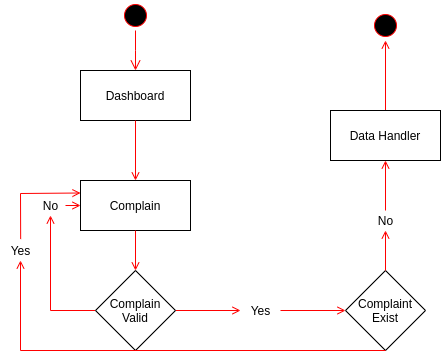
\includegraphics[scale=0.3]{img/State Diagram1.png}    
    \caption{Complaint State Diagram}
\end{figure}

\noindent The decisions that takes place in Figure 3 are the identification 
of validity of the complaint and checking if complaint already exists, 
else the process is straight forward.\\
\begin{figure}[h]
    \centering
    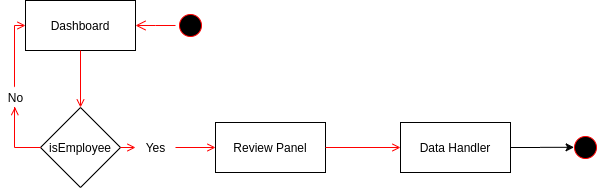
\includegraphics[scale=0.3]{img/State Diagram2.png}    
    \caption{Review State Diagram}
\end{figure}

\noindent The decision that takes place in Figure 4 is the verification of the fact 
that the person accessing the panel is an employee.\\
\begin{figure}[h]
    \centering
    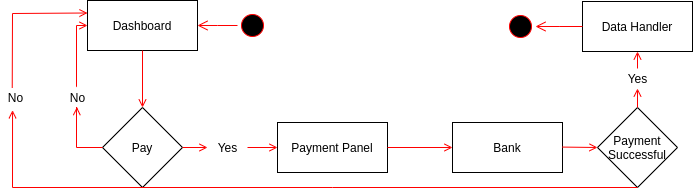
\includegraphics[scale=0.3]{img/State Diagram3.png}    
    \caption{Payment State Diagram}
\end{figure}

\noindent The decision that takes place in Figure 5 is the conformation from the 
bank is the status of transaction.\\ 
\begin{figure}[h]
    \centering
    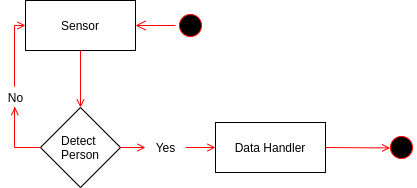
\includegraphics[scale=0.3]{img/State Diagram4.png}    
    \caption{Sensor State Diagram}
\end{figure}

\noindent The decision that takes place in Figure 6 is if the sensor does detect 
a person or a vehicle.
\section*{Conclusion and Future Work}
This is the significant part of your research paper, where you design the 
software system and explain its overall architecture. You should explain 
the pipeline of your system, about the various interactions between the model, 
view and the controller, how the database is being updated etc. We expect a neat 
design that eloquently explains your system. Use classic software design principles 
for this, listing down the use cases and making use of UML sequence, state and 
class diagrams. You should present a nice blueprint of your system and convince 
the reader that it’s an effective system and would have a high probability of 
succeeding in the real world.

Conclude well and summarise your solution in 3-4 sentences. 
Talk about future work and how things can be improved in the coming times.

\section*{References}
Sources :
\begin{itemize}
    \item \href{https://www.apple.com/in/newsroom/2020/04/apple-and-google-partner-on-covid-19-contact-tracing-technology/}{Apple and Goole Collaboration}
    \item \href{https://science.sciencemag.org/content/368/6489/409}{Finding cure of Corona Virus using structural similarity}
    \item \href{https://www.thehindu.com/sci-tech/science/how-does-soap-use-help-in-tackling-covid-19/article31070630.ece}{Soap as a protection against Corona Virus}
\end{itemize}

\end{document}
